This guide covers every feature of \app{}, grouped by task. All shortcuts are listed
in Section~\ref{sec:shortcuts}, and Section~\ref{sec:calculation} explains the
calculation.

% =====================================================================
\subsection{Projects and Files}\label{sec:files}

\subsubsection{Creating, opening and saving layouts}

A \emph{layout} is a complete study saved as a single JSON file
(Appendix~\ref{app:formats}). It contains:
\begin{itemize}
  \item the equipment and its properties;
  \item positions, sizes, rotations and bus nodes;
  \item the wiring and the grid settings;
  \item the Equipment Library;
  \item the zone settings and verification state;
  \item the path of the background PDF.
\end{itemize}
Opening a layout restores the drawing exactly as it was saved.

\begin{table}[H]
  \centering
  \caption{Layout commands (File tab)}
  \label{tab:filecommands}
  \begin{tabularx}{\textwidth}{l l L}
    \toprule
    \textbf{Command} & \textbf{Shortcut} & \textbf{What it does} \\
    \midrule
    New & \keys{Ctrl + N} & Starts an empty, untitled layout. \\
    Open & \keys{Ctrl + O} & Opens a saved layout and loads its equipment into the library. \\
    Save & \keys{Ctrl + S} & Saves to the current file, or asks for a file name the first time. \\
    Save As & \keys{Ctrl + Shift + S} & Saves to a new file. \\
    \bottomrule
  \end{tabularx}
\end{table}

If the layout has unsaved changes when you choose New or Open, or close the window,
the tool asks whether to \ui{Save}, \ui{Discard} or \ui{Cancel}. While changes are
unsaved, the window title shows an asterisk.

\subsubsection{Importing a PDF background}

\menu{File > Import PDF} shows the first page of a PDF under the drawing. The page is
drawn at true scale to match the grid, so a standard $48 \times 36$ inch sheet fills
the workspace. \menu{View > Show PDF} hides or shows it.

The layout stores the PDF's file path, not a copy of the PDF, so keep the PDF with the
project. If the PDF has moved or cannot be read when you open the layout, the tool
asks you to find it. Choose \ui{Cancel} to open the drawing without its background.

\subsubsection{Importing a netlist}

\menu{File > Import Netlist} reads a netlist JSON file (Appendix~\ref{app:formats})
and builds a drawing from its components and connections. This \emph{replaces} the
current drawing, along with its background PDF, zones and settings, so the tool asks
you to confirm first. If the file is invalid, the tool explains why and leaves the
current drawing unchanged.

\subsubsection{Exporting}

\menu{File > Export Results} offers two PDFs, described in Section~\ref{sec:reports}:
\begin{itemize}
  \item \ui{Save Calculation PDF}, the study results; and
  \item \ui{Netlist PDF}, the component and connection list.
\end{itemize}
\ui{Export Results} is available once an evaluation has been run. If you have changed
the drawing since then, run the evaluation again before exporting.

% =====================================================================
\subsection{Building the One-Line Diagram}\label{sec:building}

\subsubsection{The equipment library and Create Component}

The \ui{Equipment Library} on the left lists the equipment you can place. A new
layout's library is empty. Entries come from two places:
\begin{itemize}
  \item \ui{Create Component} on the Edit tab, which adds a new entry; and
  \item opening a layout, which adds each different component in it, with its saved
        settings. Identical components are listed once.
\end{itemize}
Type in the search box above the list to filter it by name.

\ui{Create Component} asks for a symbol type and a name, which defaults to the symbol
type. It shows only the fields that apply to that type (Figure~\ref{fig:create},
Table~\ref{tab:createfields}).

\begin{figure}[H]
  \centering
  \begin{subfigure}[t]{0.32\textwidth}\centering
    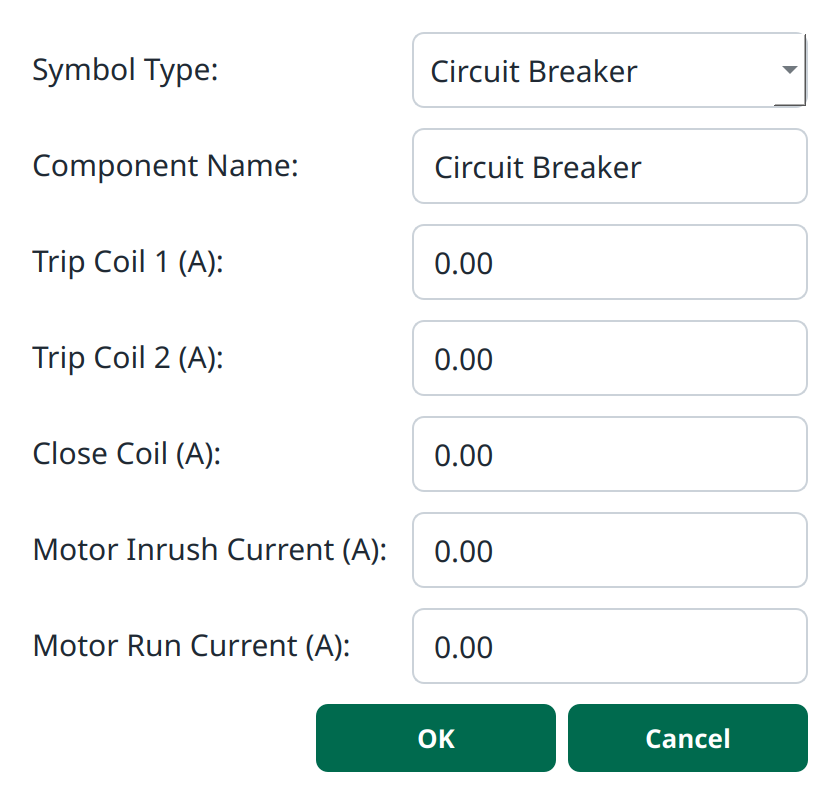
\includegraphics[width=\textwidth]{images/create_breaker.png}\caption{Circuit breaker}\end{subfigure}\hfill
  \begin{subfigure}[t]{0.32\textwidth}\centering
    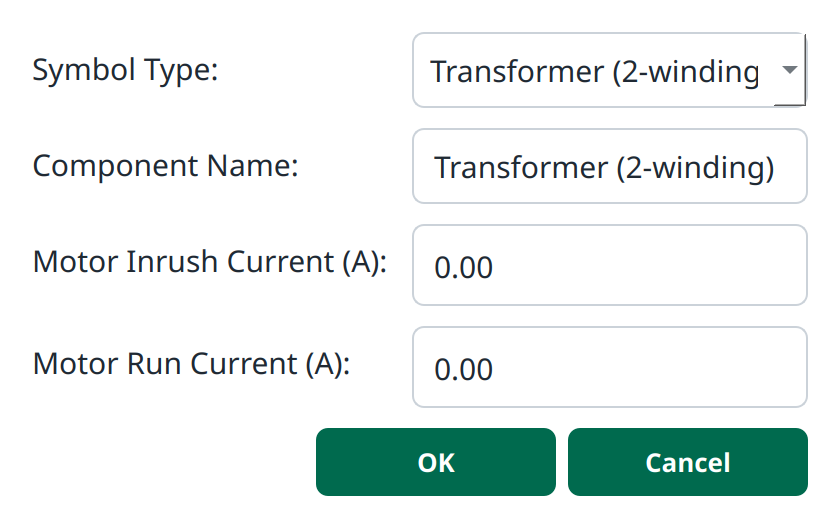
\includegraphics[width=\textwidth]{images/create_xfmr_2w.png}\caption{Transformer}\end{subfigure}\hfill
  \begin{subfigure}[t]{0.32\textwidth}\centering
    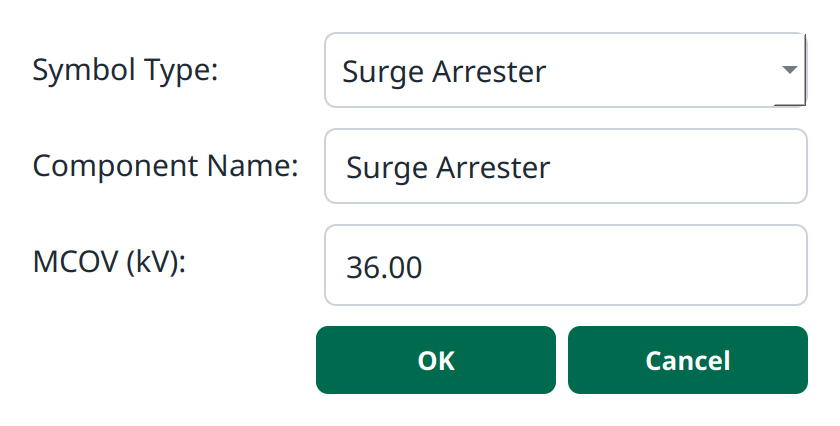
\includegraphics[width=\textwidth]{images/create_surge_arrester.png}\caption{Surge arrester}\end{subfigure}
  \caption{The Create Component dialog shows only the fields for the chosen symbol}
  \label{fig:create}
\end{figure}

\begin{table}[H]
  \centering
  \caption{Fields offered by Create Component}
  \label{tab:createfields}
  \begin{tabularx}{\textwidth}{>{\raggedright\arraybackslash}p{5.6cm} L}
    \toprule
    \textbf{Symbol type} & \textbf{Fields} \\
    \midrule
    Circuit Breaker, Custom & Trip Coil 1, Trip Coil 2, Close Coil, Motor Inrush and Motor Run currents (A) \\
    Motor Operated Switch & Motor Inrush and Motor Run currents (A) \\
    Transformer (2- and 3-winding), Potential Transformer & Motor Inrush and Motor Run currents (A). These are recorded for reference and are \emph{not} included in the DC calculation. \\
    Bus & Rating (kV) \\
    Surge Arrester & MCOV, the maximum continuous operating voltage (kV) \\
    Disconnect Switch, Current Transformer, Line Trap, Incoming AC Line, Ground & None \\
    \bottomrule
  \end{tabularx}
\end{table}

Figure~\ref{fig:symbols} shows every symbol. Junctions are not in the library; the
tool adds one automatically when you connect a wire into another wire.

\begin{figure}[H]
  \centering
  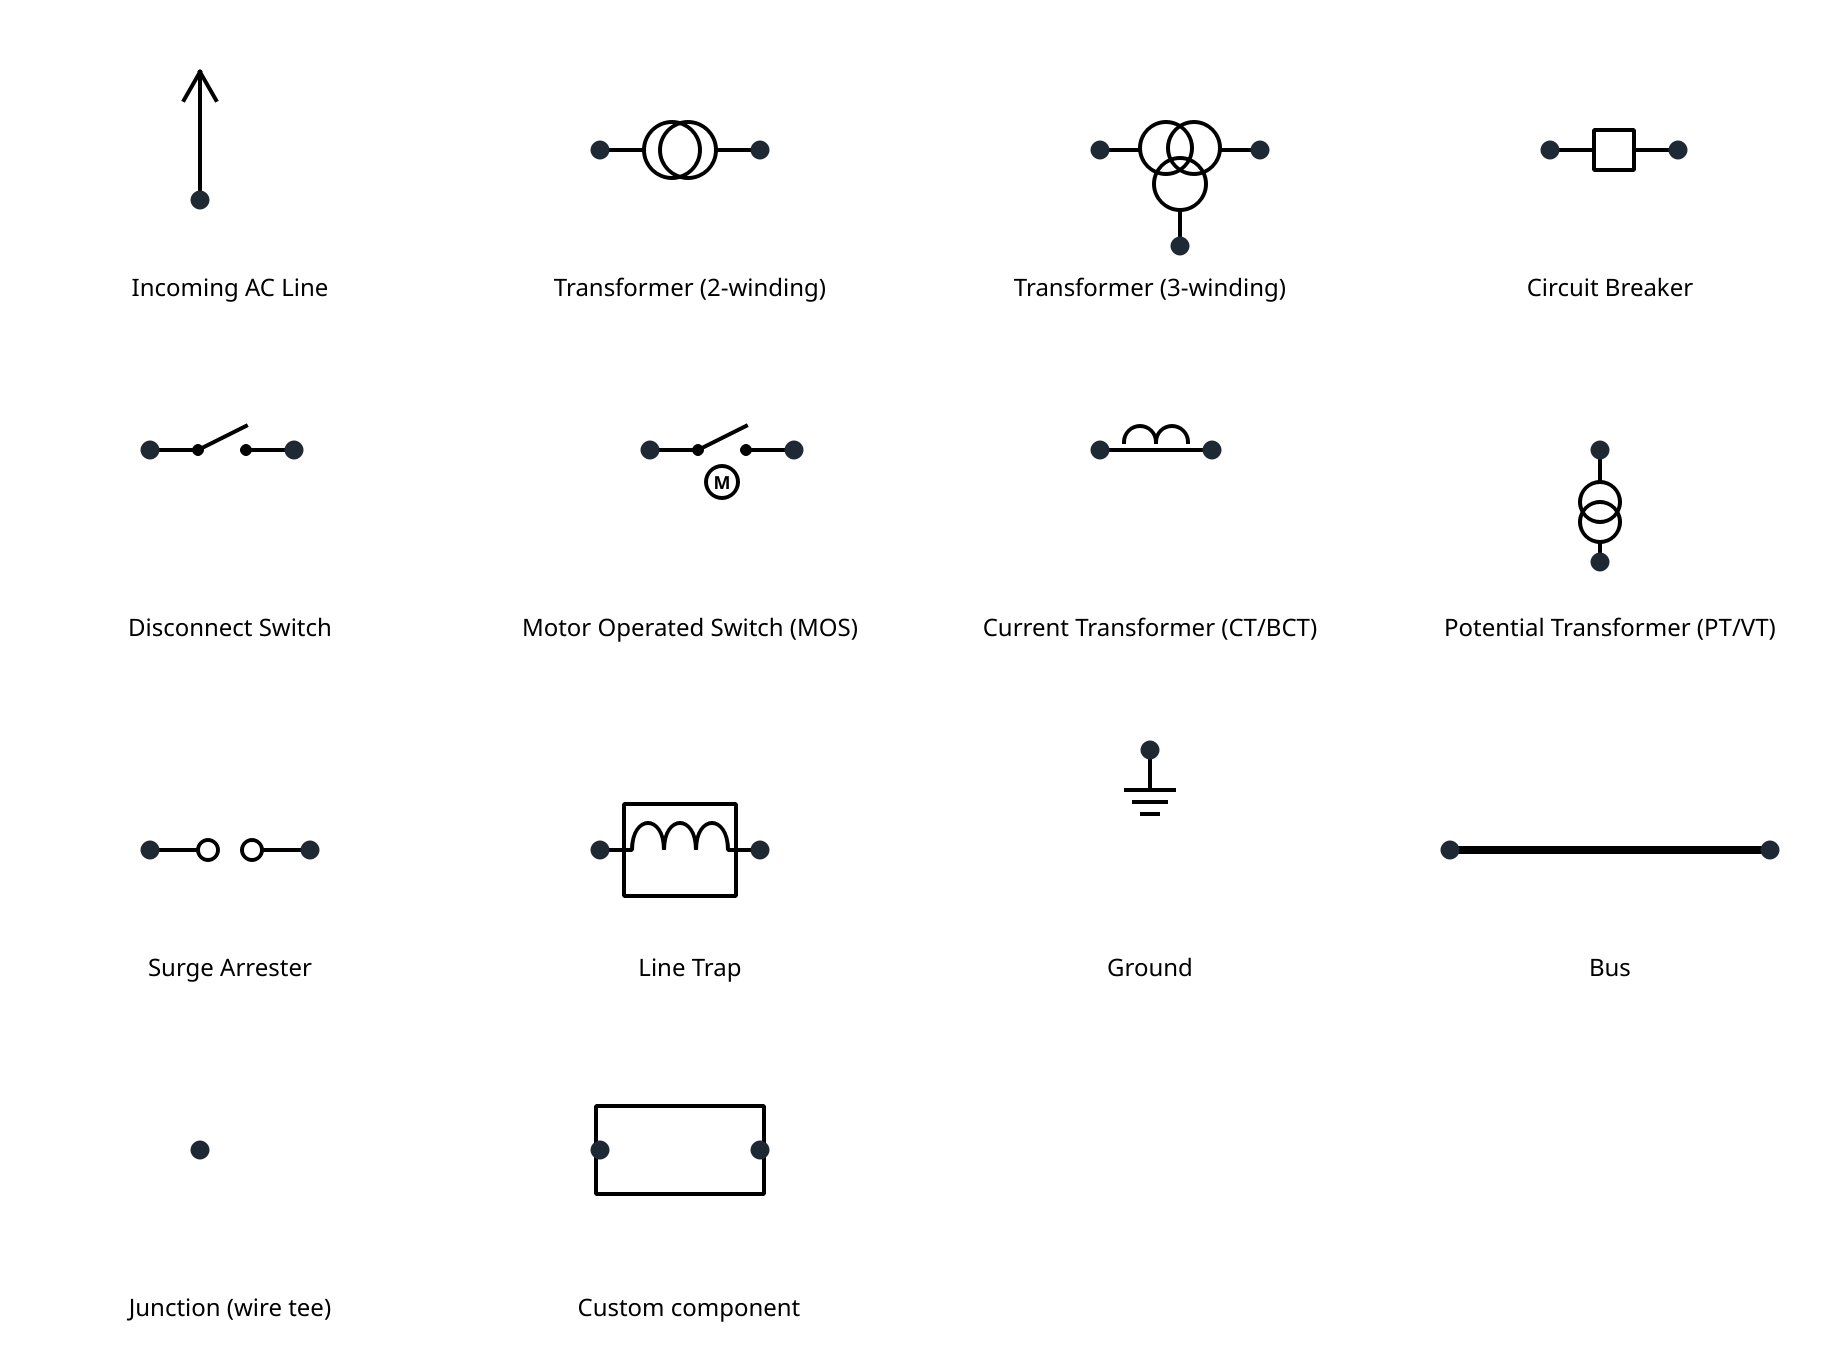
\includegraphics[width=0.9\textwidth]{images/symbol_gallery.png}
  \caption{Equipment symbols. The dark dots are terminals.}
  \label{fig:symbols}
\end{figure}

\subsubsection{Placing equipment}

Drag an entry from the library onto the drawing. A preview follows the pointer, and
the equipment is placed where you release it. With \ui{Snap to Grid} on (the default),
its terminals snap to the nearest grid point so that wires line up. Grid lines are
half an inch apart.


Each placed copy gets its own ID, which is shown beside the symbol and used in the
results and reports. You can change it in the properties panel.

\subsubsection{Connecting equipment}\label{sec:connecting}

Wires connect \emph{terminals}, the dark dots on each symbol, and route themselves at
right angles. Wires that only cross on the drawing are \emph{not} connected.

\begin{description}[style=nextline, leftmargin=1.2em]
  \item[Terminal to terminal]
    Press the mouse button on a terminal, drag to another terminal and release.
  \item[To a bus]
    Release the wire anywhere along a bus bar. The tool adds a connection node there,
    or reuses a node close by. A bus can have any number of nodes.
  \item[Into an existing wire (tee)]
    Release the wire on another wire. The tool splits that wire and adds a junction
    joining all three.
  \item[Cancelling]
    Press \keys{Esc} or right-click while dragging a wire.
\end{description}

\subsubsection{Arranging the drawing}

\begin{table}[H]
  \centering
  \caption{Editing actions}
  \label{tab:editing}
  \begin{tabularx}{\textwidth}{l L}
    \toprule
    \textbf{Action} & \textbf{How} \\
    \midrule
    Select & Click a symbol or wire. \keys{Ctrl}-click adds to or removes from the selection. \\
    Move & Drag the selected equipment. Connected wires follow. \\
    Rotate & \ui{Rotate 90°} on the Edit tab, or \keys{R} and \keys{Shift + R}. You can also drag the round handle above a selected symbol; it turns in \SI{15}{\degree} steps, or freely while you hold \keys{Shift}. \\
    Resize & Drag a corner handle of a selected symbol. Sizes range from half to three times normal, in steps of 0.25. \\
    Resize a bus & Drag either end of the bus bar. A bus cannot be shortened past its connection nodes. \\
    Copy and paste & \keys{Ctrl + C} and \keys{Ctrl + V}, or the Edit tab. \\
    Delete & \keys{Delete}, \keys{Backspace} or the Edit tab. Wires attached to deleted equipment are deleted too, along with any bus nodes no longer in use. \\
    Align to Grid & On the View tab. Snaps the selected equipment to the grid, or the whole drawing if nothing is selected. \\
    Undo and redo & \keys{Ctrl + Z} and \keys{Ctrl + Y}, or the Edit tab. Every edit can be undone, including property changes and zone settings. \\
    \bottomrule
  \end{tabularx}
\end{table}

\paragraph{Copy and paste.} Copies keep their properties, breaker settings, bus nodes,
sizes and rotations, and the wires \emph{between} the copied components. Wires to
anything that was not copied are dropped. Each paste is offset from the original, gets
new IDs and numbered names such as \emph{CB-A (2)}, and undoes as a single step. Zone
assignments are not copied, so check the zones after pasting.

\subsubsection{View options}

The View tab controls what the workspace shows, without changing the study:
\begin{itemize}
  \item \ui{Show Grid}, \ui{Show PDF}, \ui{Show Circuit} and \ui{Show Zones} show or
        hide the grid, the background, the drawn equipment and the zone outlines;
  \item \ui{Snap to Grid} turns snapping on or off;
  \item the \ui{Grid Opacity} slider sets how dark the grid lines are.
\end{itemize}
Hold \keys{Ctrl} and turn the mouse wheel to zoom, and drag an empty part of the
drawing to pan.

% =====================================================================
\subsection{Equipment Properties}\label{sec:properties}

Selecting one component shows its data in the \ui{Selected Element Properties} panel
(Figure~\ref{fig:properties}). The fields depend on the component type:
\begin{itemize}
  \item breakers and custom components show all five currents and the breaker settings;
  \item transformers and potential transformers show only their motor currents;
  \item buses show their voltage, and surge arresters their MCOV.
\end{itemize}

\begin{figure}[H]
  \centering
  \begin{subfigure}[t]{0.48\textwidth}\centering
    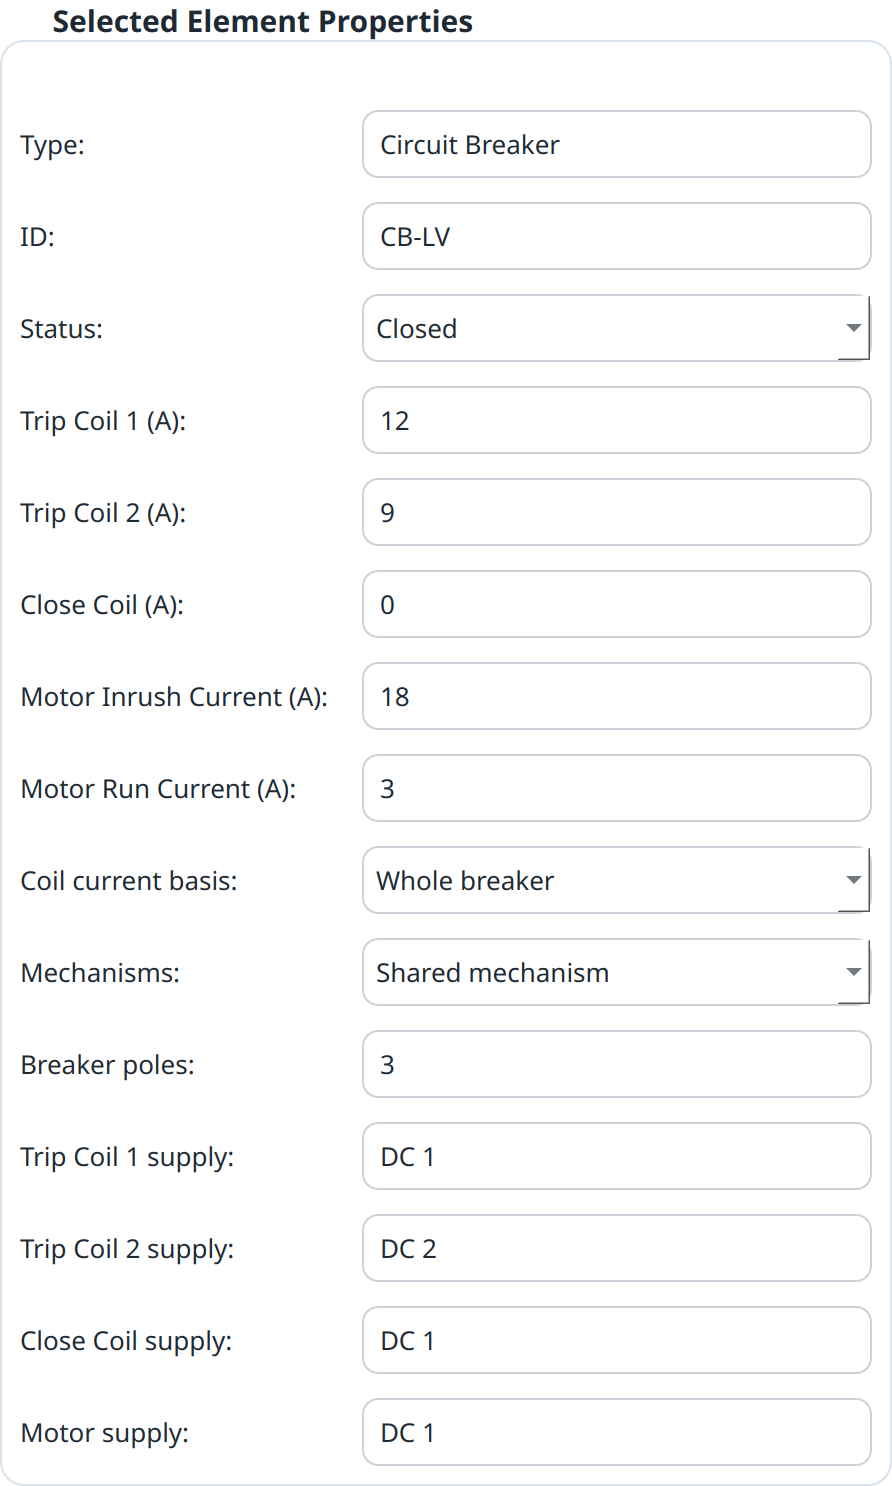
\includegraphics[width=\textwidth]{images/properties_breaker.png}
    \caption{Circuit breaker, with breaker settings}\end{subfigure}\hfill
  \begin{subfigure}[t]{0.48\textwidth}\centering
    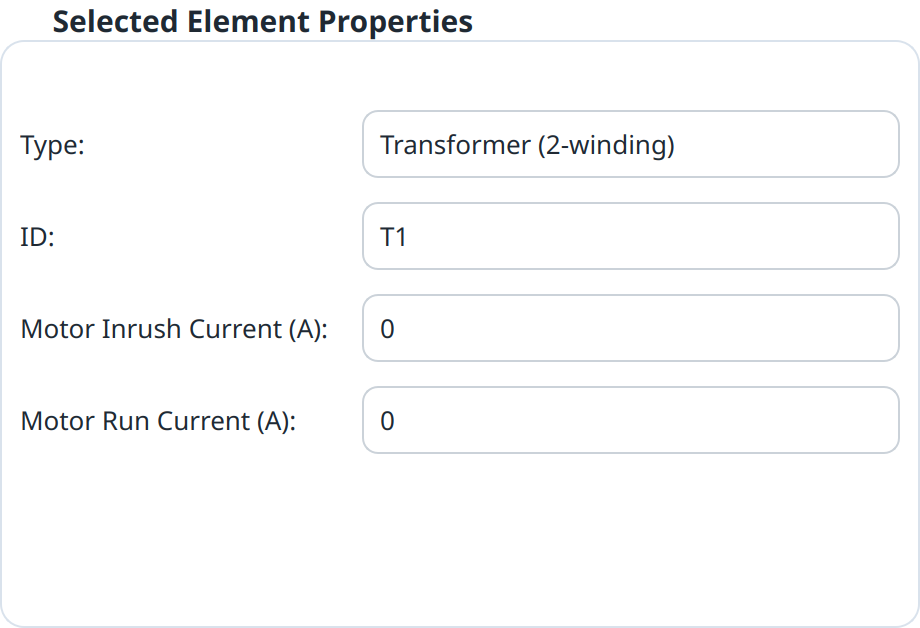
\includegraphics[width=\textwidth]{images/properties_transformer.png}
    \caption{Transformer}\vspace{6pt}
    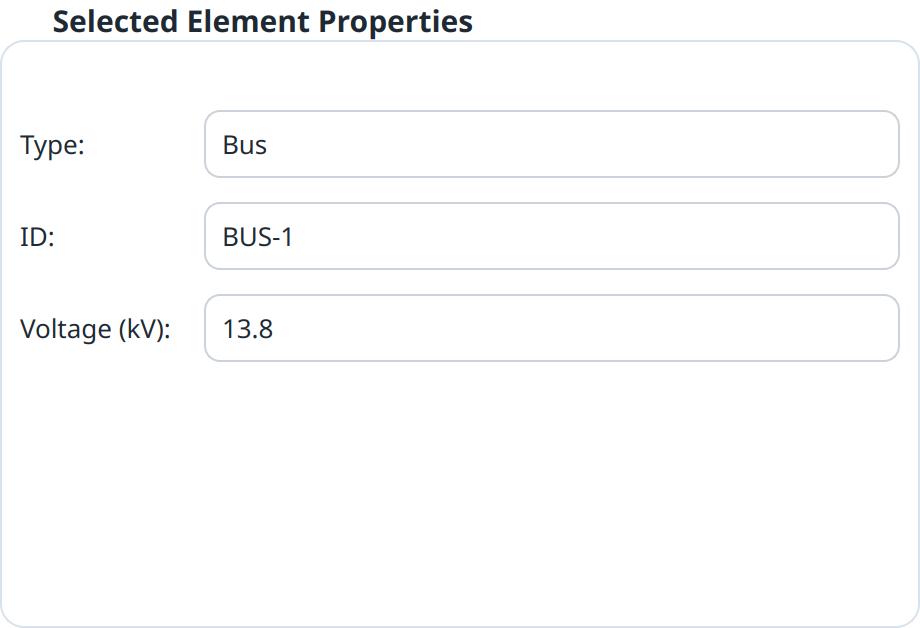
\includegraphics[width=\textwidth]{images/properties_bus.png}
    \caption{Bus}\end{subfigure}
  \caption{The properties panel for different equipment}
  \label{fig:properties}
\end{figure}

Rules for editing:
\begin{itemize}
  \item An edit takes effect when you press \keys{Enter} or leave the field. It can be
        undone.
  \item A blank current counts as zero. Currents must be zero or positive, and a bus
        voltage must be positive or blank. An invalid entry is not applied, and the
        status bar explains why.
  \item Edits change only the selected component, not the library entry it came from.
\end{itemize}

\paragraph{Status.} Switching devices have a status, which affects zone detection
(Table~\ref{tab:status}).

\begin{table}[H]
  \centering
  \caption{Status values}
  \label{tab:status}
  \begin{tabularx}{\textwidth}{l L}
    \toprule
    \textbf{Status} & \textbf{Effect on zone detection} \\
    \midrule
    Closed (default) & Conducts normally. \\
    Open & On a breaker, disconnect switch or motor-operated switch, splits the drawing at the device. Open breakers are not suggested as trip breakers. \\
    Normally Open & Same as Open. Use it for normally open bypass switches, so that they do not join bus sections. \\
    Maintenance & For reference only; the device is treated as closed. \\
    \bottomrule
  \end{tabularx}
\end{table}

\paragraph{Breaker settings.} Below its currents, a breaker has settings that apply
wherever it operates (Table~\ref{tab:breakersettings}). They determine how many coils
operate together and which DC supply feeds each coil
(Section~\ref{sec:calcmultipliers}).

\begin{table}[H]
  \centering
  \caption{Breaker settings}
  \label{tab:breakersettings}
  \begin{tabularx}{\textwidth}{>{\raggedright\arraybackslash}p{3.2cm} >{\raggedright\arraybackslash}p{3.6cm} L}
    \toprule
    \textbf{Setting} & \textbf{Options} & \textbf{Meaning} \\
    \midrule
    Coil current basis & Whole breaker / Per mechanism & Whether the entered coil currents are for the whole breaker or for each pole's mechanism. \\
    Mechanisms & Shared mechanism / Independent per pole & Whether the poles share one operating mechanism or each has its own. \\
    Breaker poles & 1 to 3 & The number of poles. \\
    Supplies (Trip Coil 1, Trip Coil 2, Close Coil, Motor) & Any name; default \emph{DC 1} & The DC supply for each coil and for the motor. Each supply is reported separately. \\
    \bottomrule
  \end{tabularx}
\end{table}

For most breakers, which have one shared mechanism and a single DC supply, the
defaults are correct.


% =====================================================================
\subsection{Validating the Drawing}\label{sec:validate}

\menu{Analysis > Validate} checks the wiring and lists any problems in a message
window, and the status bar shows the counts, for example
\emph{Circuit check: 1 open, 0 short}. It does not change the drawing.

\begin{table}[H]
  \centering
  \caption{Validate messages}
  \label{tab:validate}
  \begin{tabularx}{\textwidth}{l L}
    \toprule
    \textbf{Message} & \textbf{Meaning and fix} \\
    \midrule
    \emph{Name: port is not connected} & A terminal has no wire. Connect it, or end the circuit with an Incoming AC Line. \\
    \emph{Name: junction is not connected} & A junction has no wires; delete it. \\
    \emph{Name: dangling wire (only one connection)} & A junction has only one wire; finish or remove the branch. \\
    \emph{Name: bus is not connected} & A bus has no wires at all. \\
    \emph{Name: A and B are on the same node} & Both sides of a two-terminal device, such as a breaker or transformer, are connected together, so the device is bypassed. \\
    \emph{Bus is tied directly to Ground} & A ground is wired straight to a bus. \\
    \emph{No components on the canvas.} & The drawing is empty. \\
    \bottomrule
  \end{tabularx}
\end{table}

% =====================================================================
\subsection{Protection Zones}\label{sec:zones}

A \emph{zone} represents one protection scheme operating for a fault: the equipment it
protects, the CTs that bound it, and the loads that operate when it trips. Zones are
saved in the layout. Only the configured zones are used in the calculation; detected
regions are shown for reference.

\subsubsection{Automatic proposals}

The first time you use \ui{Run Evaluation} or \ui{Configure Zones} on a layout without
zones, the tool proposes bus, transformer and line zones by tracing the wiring. It
follows these rules:

\begin{itemize}
  \item Proposals follow actual wires, junctions and terminals, and stop at CTs. A CT
        is a boundary: one side is inside the zone, the other outside.
  \item Open and normally open breakers, disconnects and motor-operated switches split
        regions. A missing or unrecognized status counts as closed.
  \item An unbranched path through one closed breaker can extend a zone to the CTs on
        the far side, so neighboring zones overlap at that breaker, as they do in
        practice.
  \item A line terminal gets a zone only if its CT-bounded region contains a closed
        breaker. Metering taps that reach other bays do not create line zones.
  \item Separate transformer zones need CTs between them. A region shared by a bus
        and a transformer does not qualify.
  \item Buses that share one region get a single proposal. Transfer buses, recognized
        by their name, stay on the drawing but never get a zone of their own.
  \item Breakers next to a zone are listed as \emph{suggested} trip breakers, stopping
        at open switches. They are not assigned as loads automatically.
\end{itemize}

Proposals never include operating loads and are never verified automatically; the
engineer always completes and confirms them.

\subsubsection{The Configure Zones dialog}

\menu{Analysis > Configure Zones} opens the zone editor (Figure~\ref{fig:zonedialog}).
The zone list is on the left. \ui{Add Zone} creates a new manual zone, and
\ui{Delete Zone} removes the selected one. The selected zone's settings are on the
right.

\begin{figure}[H]
  \centering
  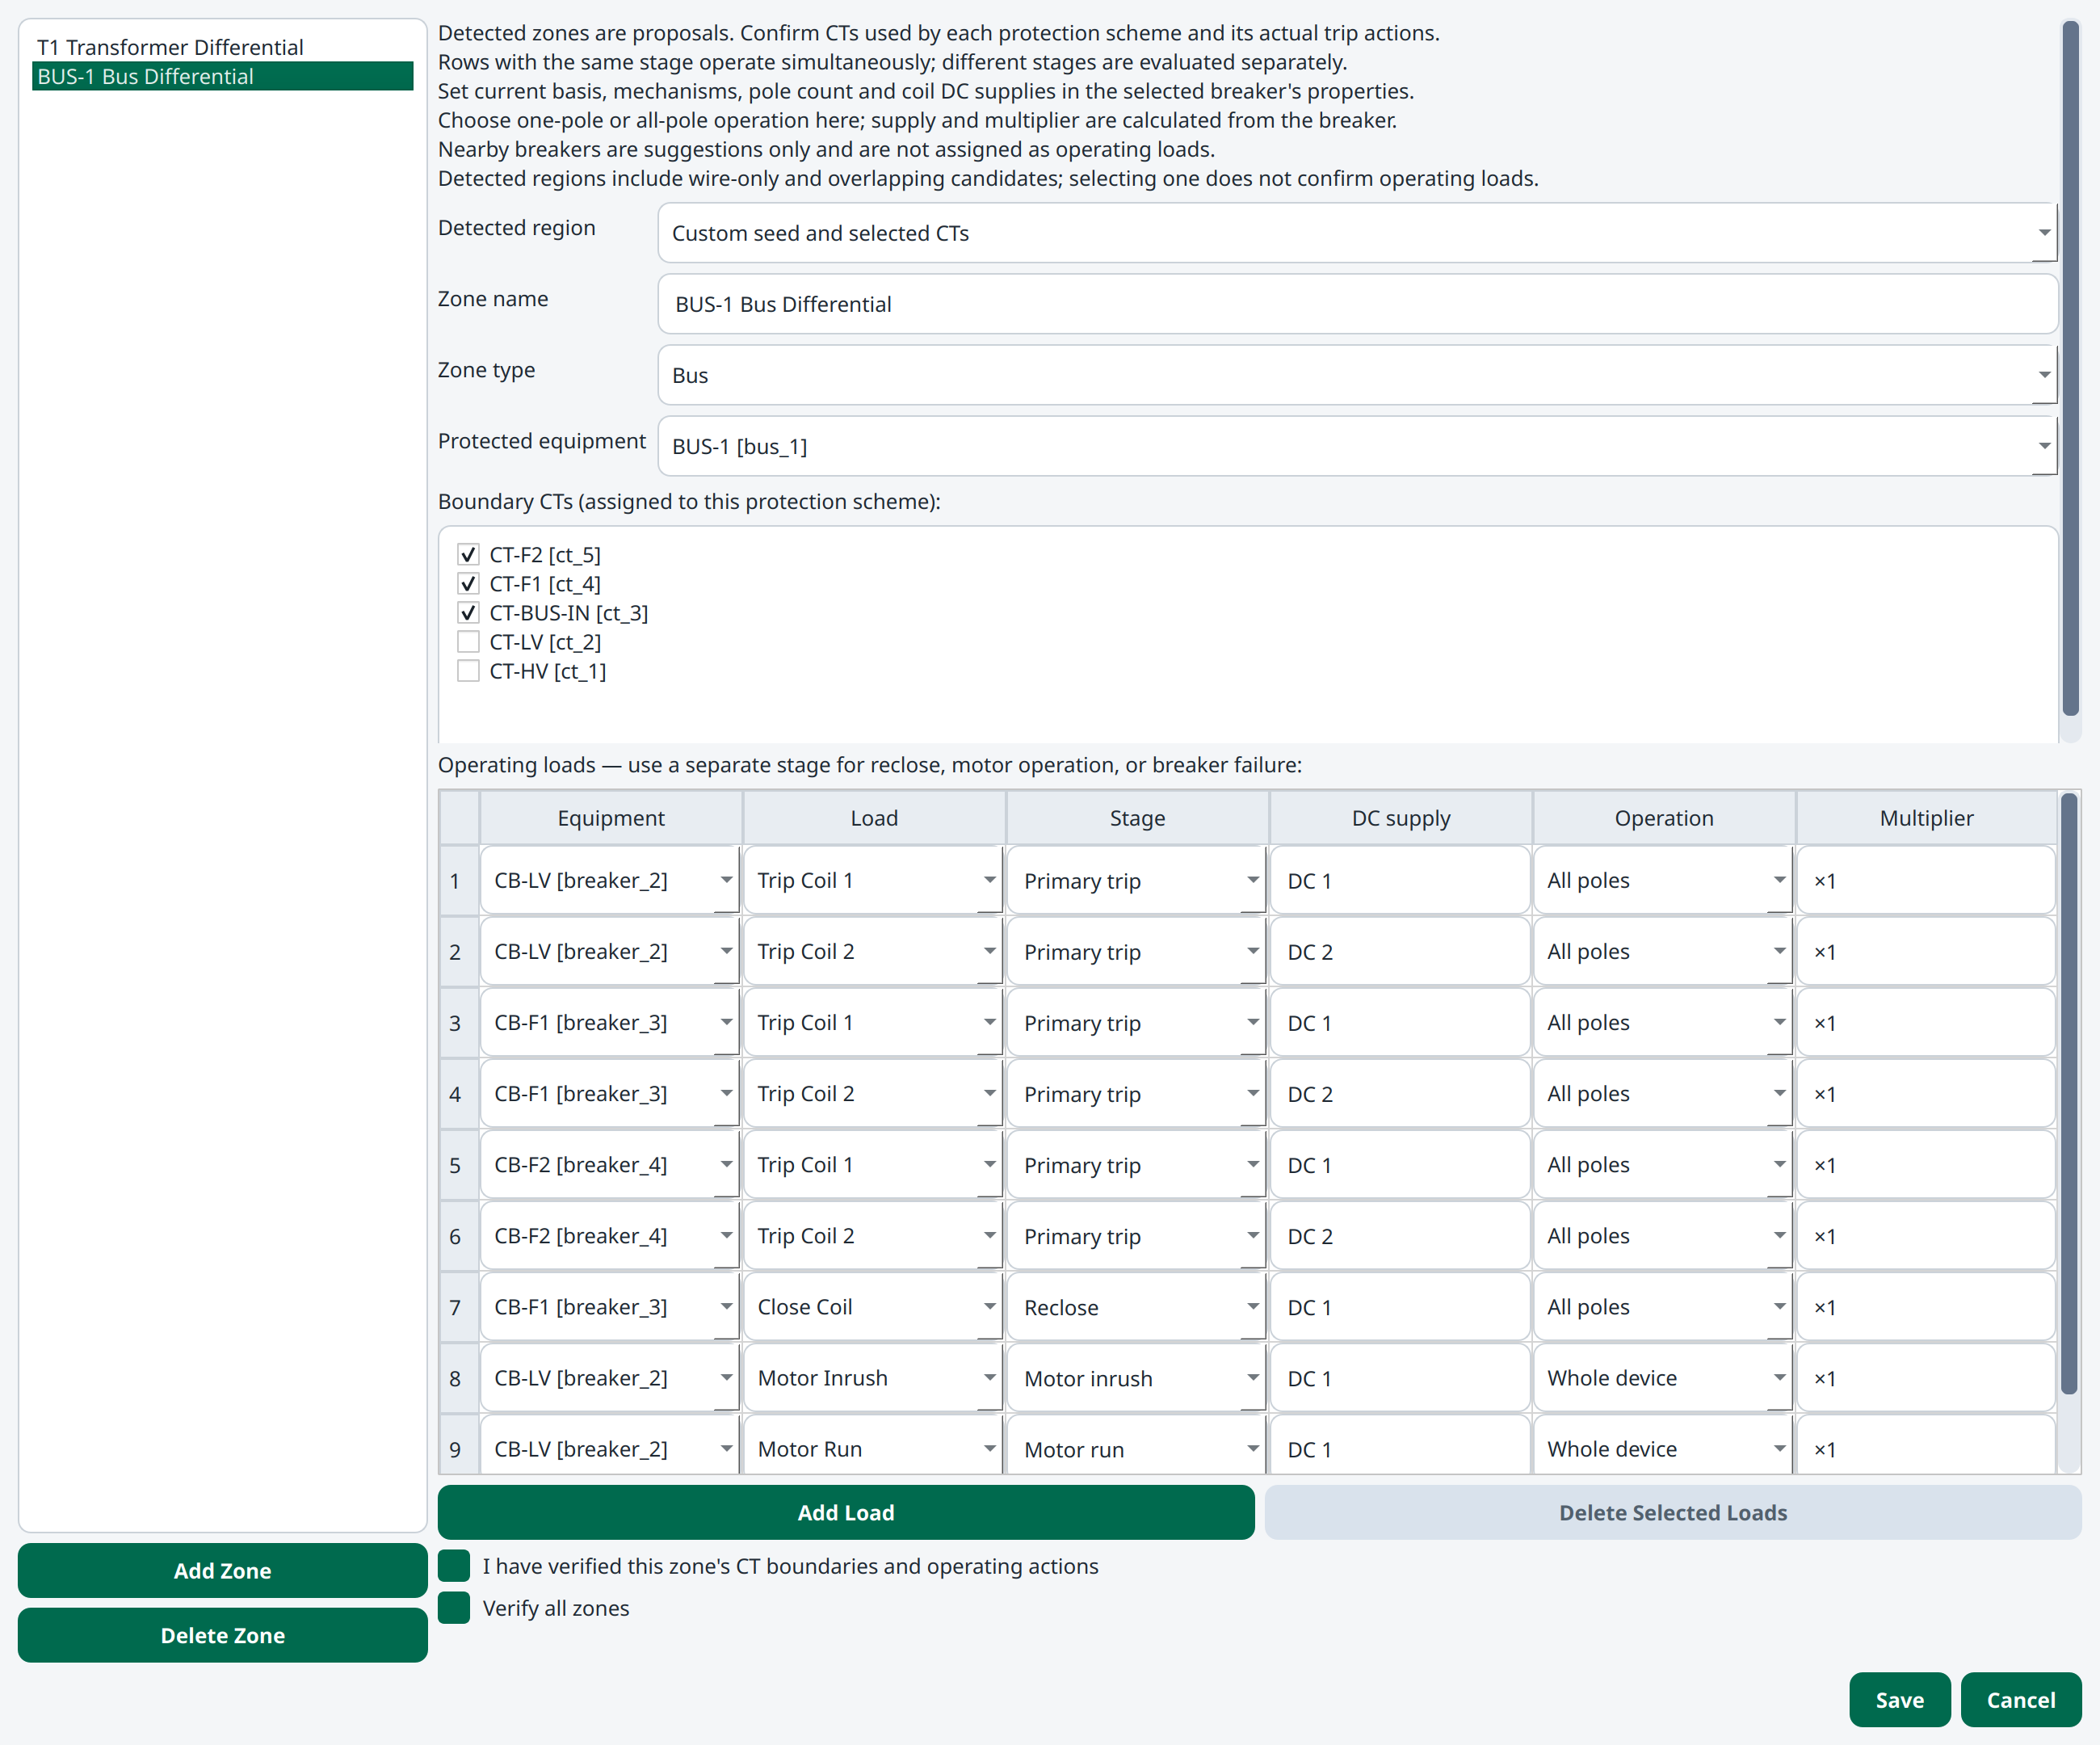
\includegraphics[width=\textwidth]{images/zone_dialog.png}
  \caption{Configure Zones, showing the verified bus zone of the two-zone demonstration}
  \label{fig:zonedialog}
\end{figure}

\begin{table}[H]
  \centering
  \caption{Zone settings}
  \label{tab:zonesettings}
  \begin{tabularx}{\textwidth}{l L}
    \toprule
    \textbf{Field} & \textbf{Purpose} \\
    \midrule
    Detected region & Choose a detected region to use its exact equipment and wiring, or \emph{Custom seed and selected CTs} to define the zone by its protected equipment and checked CTs. \\
    Zone name & Shown in the results and the report. \\
    Zone type & Bus, Transformer, Line or Manual. \\
    Protected equipment & The bus, transformer or other device the zone is built around. \\
    Boundary CTs & Check only the CTs this scheme uses; leave metering CTs and other schemes' CTs unchecked. Zones may overlap and share equipment. \\
    \bottomrule
  \end{tabularx}
\end{table}

\subsubsection{Operating loads}

The table at the bottom of the dialog lists what operates when the zone trips. Each
row is one coil or motor; \ui{Add Load} adds a row.

\begin{table}[H]
  \centering
  \caption{Operating-load columns}
  \label{tab:loadcolumns}
  \begin{tabularx}{\textwidth}{l L}
    \toprule
    \textbf{Column} & \textbf{Meaning} \\
    \midrule
    Equipment & The device that operates, or \emph{Other} for a load not on the drawing. Passive equipment, such as CTs, buses and transformers, is not listed. \\
    Load & Trip Coil 1, Trip Coil 2, Close Coil, Motor Inrush or Motor Run. For \emph{Other}, type the current in amperes instead. \\
    Stage & When the load operates (Table~\ref{tab:stages}). Rows in the same stage operate at the same time. \\
    DC supply & For breakers, taken from the breaker settings and read-only. For other devices, editable. \\
    Operation & \emph{All poles} or \emph{One pole} for breaker coils; \emph{Whole device} for motors and other equipment. \\
    Multiplier & Read-only: how many coils operate (Section~\ref{sec:calcmultipliers}). \\
    \bottomrule
  \end{tabularx}
\end{table}

\begin{table}[H]
  \centering
  \caption{Operating stages}
  \label{tab:stages}
  \begin{tabularx}{\textwidth}{l L}
    \toprule
    \textbf{Stage} & \textbf{Typical use} \\
    \midrule
    Primary trip & The zone's own breakers trip. Assign Trip Coil 2 here as well if both coils operate together. \\
    Backup trip & Backup protection operates. If its loads overlap the primary trip in time, put them in the primary trip stage instead. \\
    Breaker failure & A breaker fails to clear and the surrounding breakers trip. \\
    Reclose & Breakers close again. \\
    Motor inrush & Spring-charging motors start. \\
    Motor run & Motors run after starting. A motor cannot be in its inrush and run stages at the same time. \\
    Background load & Added automatically when a zone has only \emph{Other} loads. \\
    \bottomrule
  \end{tabularx}
\end{table}

\paragraph{Other loads.} Choose \emph{Other} as the equipment for a continuous load
that is not on the drawing, such as relay or panel load, and type its current. Other
loads are treated as standing current on \emph{DC 1} and added to \emph{every} stage of
the zone. For example, a \SI{10}{A} trip stage with a \SI{5}{A} Other load totals
\SI{15}{A}.


\paragraph{Selecting and deleting rows.} Click the row numbers to select rows.
\keys{Shift}-click selects a range, and \keys{Ctrl}-click adds or removes a single
row. \ui{Delete Selected Loads}, \keys{Delete} or \keys{Backspace} removes the
selected rows after you confirm. While you are typing in a cell, these keys edit the
text as usual.

\subsubsection{Verifying zones}

When you have reviewed a zone's CTs and loads, check \ui{I have verified this zone's
CT boundaries and operating actions}. \ui{Verify all zones} checks every zone that has
no outstanding issues and leaves the others as drafts; hover over it to see why.
\ui{Save} applies the changes and runs the evaluation again, and \ui{Cancel} discards
every change made in the dialog.

A verified zone must be complete. If it still has problems, \ui{Save} lists them and
does not save; clear the check box to save the zone as a draft.

Verification lapses when things change:
\begin{itemize}
  \item editing a zone in the dialog clears its check box;
  \item changing the wiring, the equipment, a switch's status or a breaker's settings
        means every verified zone must be confirmed again, because it was verified
        against the old drawing. Until then, the study is incomplete.
\end{itemize}

% =====================================================================
\subsection{Evaluation and Results}\label{sec:results}

\menu{Analysis > Run Evaluation} calculates every zone and shows the results in
\ui{Analysis Output} on the right. The status bar shows how long it took, usually
well under a tenth of a second. Any later change to the drawing clears the results.

\subsubsection{Zone outlines and the zone selector}

After an evaluation, each zone is outlined on the drawing, following its equipment and
wiring (Figure~\ref{fig:outlines}). Each zone has its own color. Dashed outlines mark
zones that are not yet complete; solid outlines mark complete, verified zones.

Use the selector above the output to show one zone or all of them. It also lists the
detected topology regions, which are drawn dotted, for reference. \ui{Show Zones} on
the View tab hides the outlines without changing the study.

\begin{figure}[H]
  \centering
  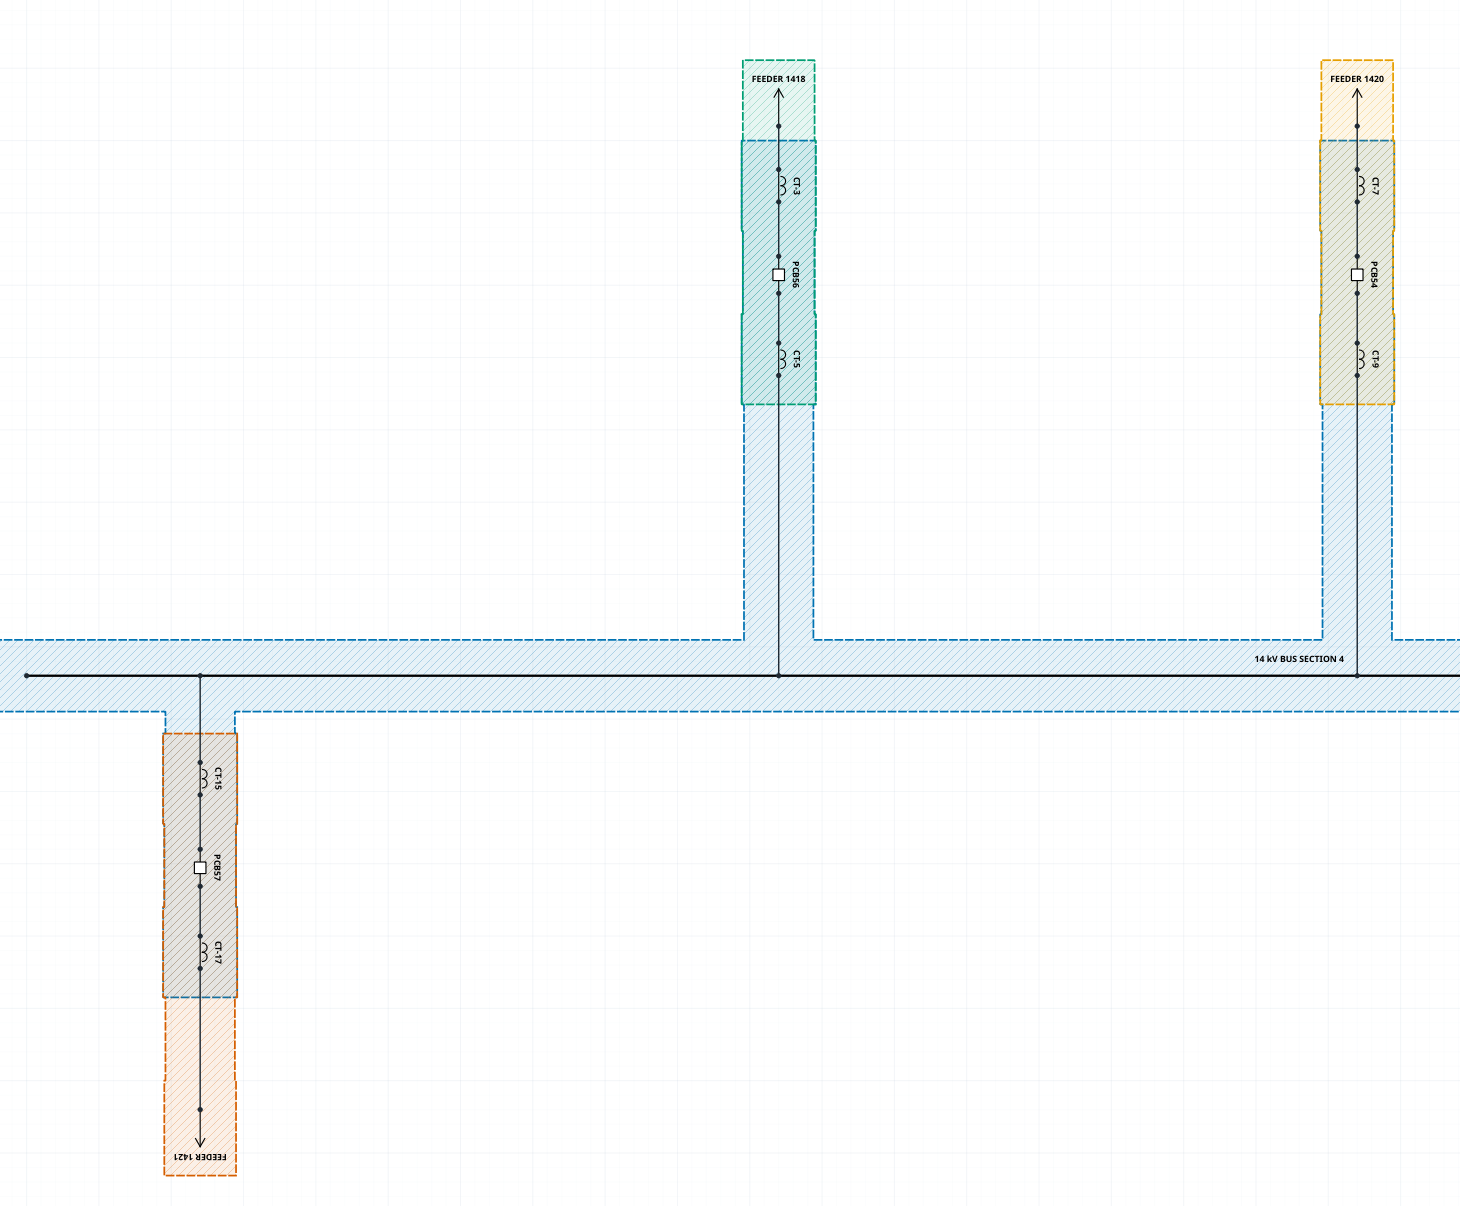
\includegraphics[width=\textwidth]{images/zone_outlines.png}
  \caption{Zone outlines on part of the AS-1 layout: the bus zone (blue) overlaps each feeder zone at its breaker. The outlines are dashed because the zones are not yet verified.}
  \label{fig:outlines}
\end{figure}

\subsubsection{The analysis output}

The output lists each zone with:
\begin{itemize}
  \item its CT boundaries and its equipment;
  \item each stage's total current, the total for each DC supply in that stage, and
        the arithmetic for every load, for example
        \emph{CB-LV - Trip Coil 1: 12 A $\times$ 1 = 12 A (DC 1)};
  \item any review warnings.
\end{itemize}
It ends with each DC supply's peak current and the zone and stage it comes from.
\menu{Analysis > Expand Analysis} opens the output in a larger, resizable window.

\subsubsection{Complete and provisional results}

A study is \textbf{COMPLETE} only when every configured zone is verified and nothing
needs review. Until then, it is \textbf{INCOMPLETE}: its totals are labeled
\emph{provisional} and the supply peaks are withheld. A study stays incomplete if, for
example, it has:

\begin{itemize}
  \item a zone that is not verified, or was verified before the drawing changed;
  \item a missing or zero current for an assigned load, or a missing DC supply;
  \item a boundary CT that is missing, not a CT, or not connected to the zone;
  \item a bus or transformer not covered by any zone;
  \item the same coil assigned to different DC supplies in different zones;
  \item a passive device assigned as a load, or a motor's inrush and run in the same
        stage.
\end{itemize}

% =====================================================================
\subsection{Reports}\label{sec:reports}

\paragraph{Calculation PDF.} \menu{File > Export Results > Save Calculation PDF}
writes the study report (Figure~\ref{fig:calcpdf}):
\begin{itemize}
  \item the study status, system name and DC voltage;
  \item the annotated one-line, showing the zone outlines as evaluated;
  \item each DC supply's peak, with its zone and stage;
  \item a zone summary of the stage totals;
  \item the review issues;
  \item the full evaluation output.
\end{itemize}
An incomplete study can still be exported, but it is marked
\textbf{INCOMPLETE --- provisional study}, and its totals are labeled provisional.

\begin{figure}[H]
  \centering
  \begin{subfigure}[t]{0.48\textwidth}\centering
    \fbox{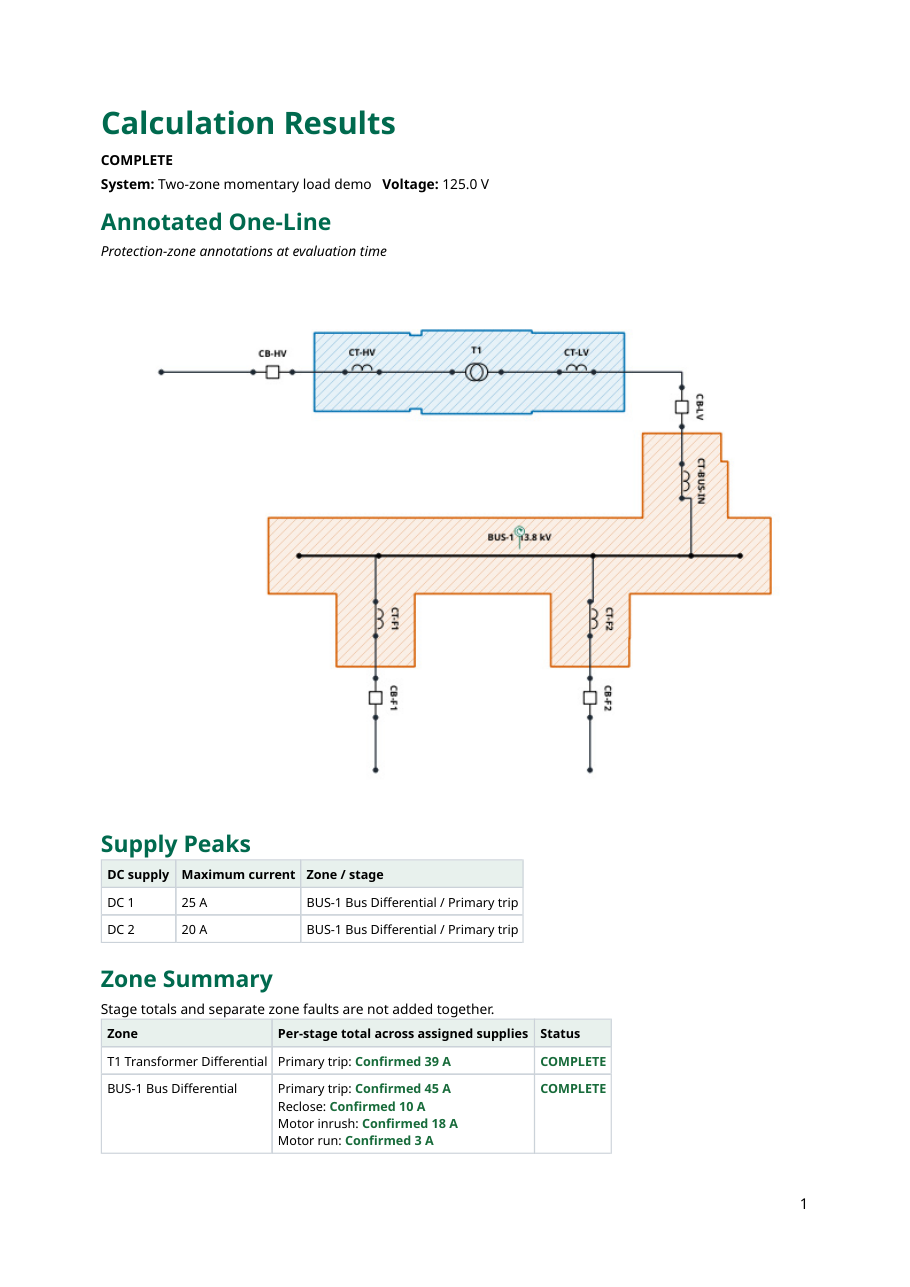
\includegraphics[width=0.97\textwidth]{images/calc_pdf_p1.png}}\caption{Page 1}\end{subfigure}\hfill
  \begin{subfigure}[t]{0.48\textwidth}\centering
    \fbox{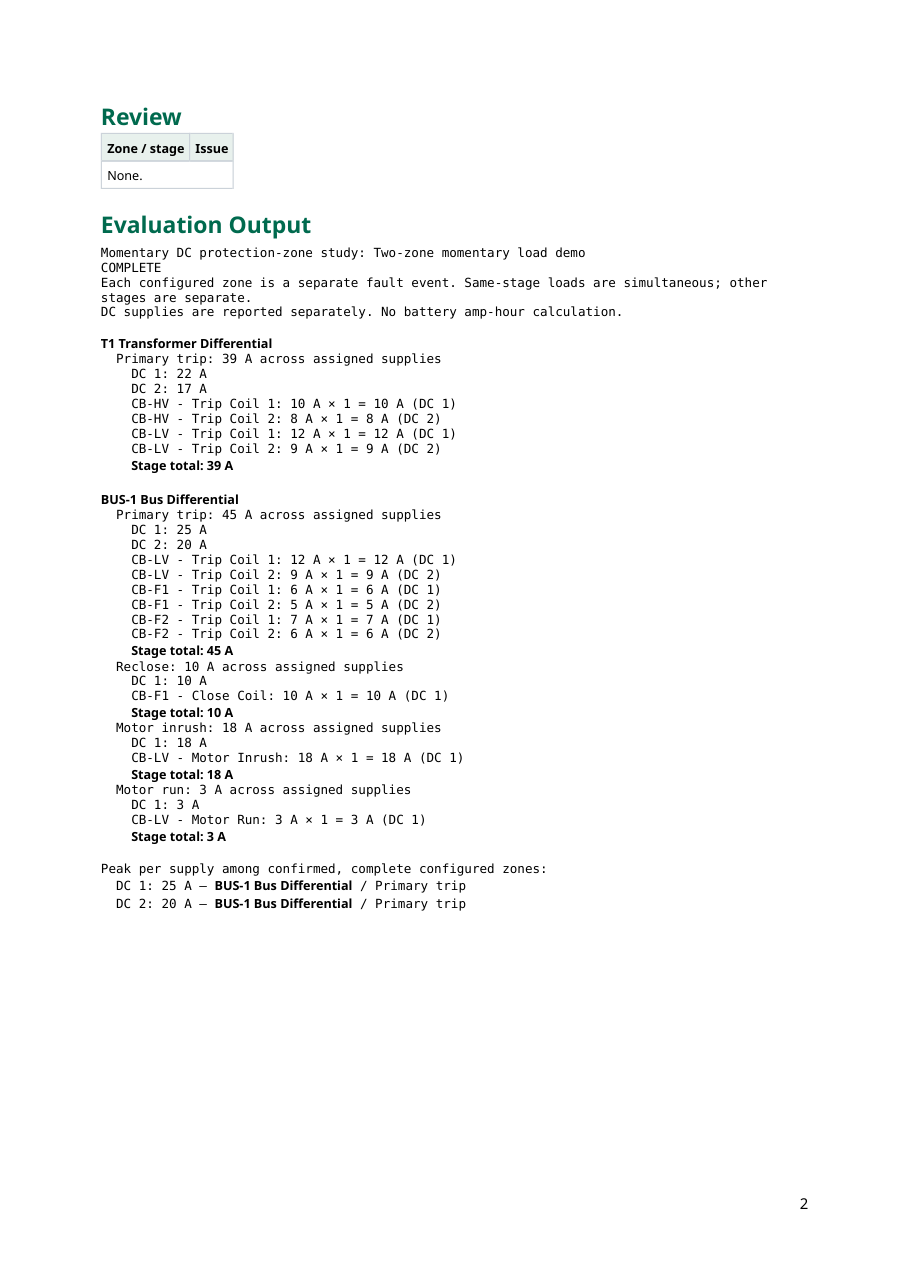
\includegraphics[width=0.97\textwidth]{images/calc_pdf_p2.png}}\caption{Page 2}\end{subfigure}
  \caption{Calculation PDF for the two-zone demonstration}
  \label{fig:calcpdf}
\end{figure}

\paragraph{Netlist PDF.} \menu{File > Export Results > Netlist PDF} lists every
component, with its ID, name, type, properties and terminals, followed by every
connection (Figure~\ref{fig:netlistpdf}). It is an inventory of the drawing for
checking against the original one-line.

\begin{figure}[H]
  \centering
  \fbox{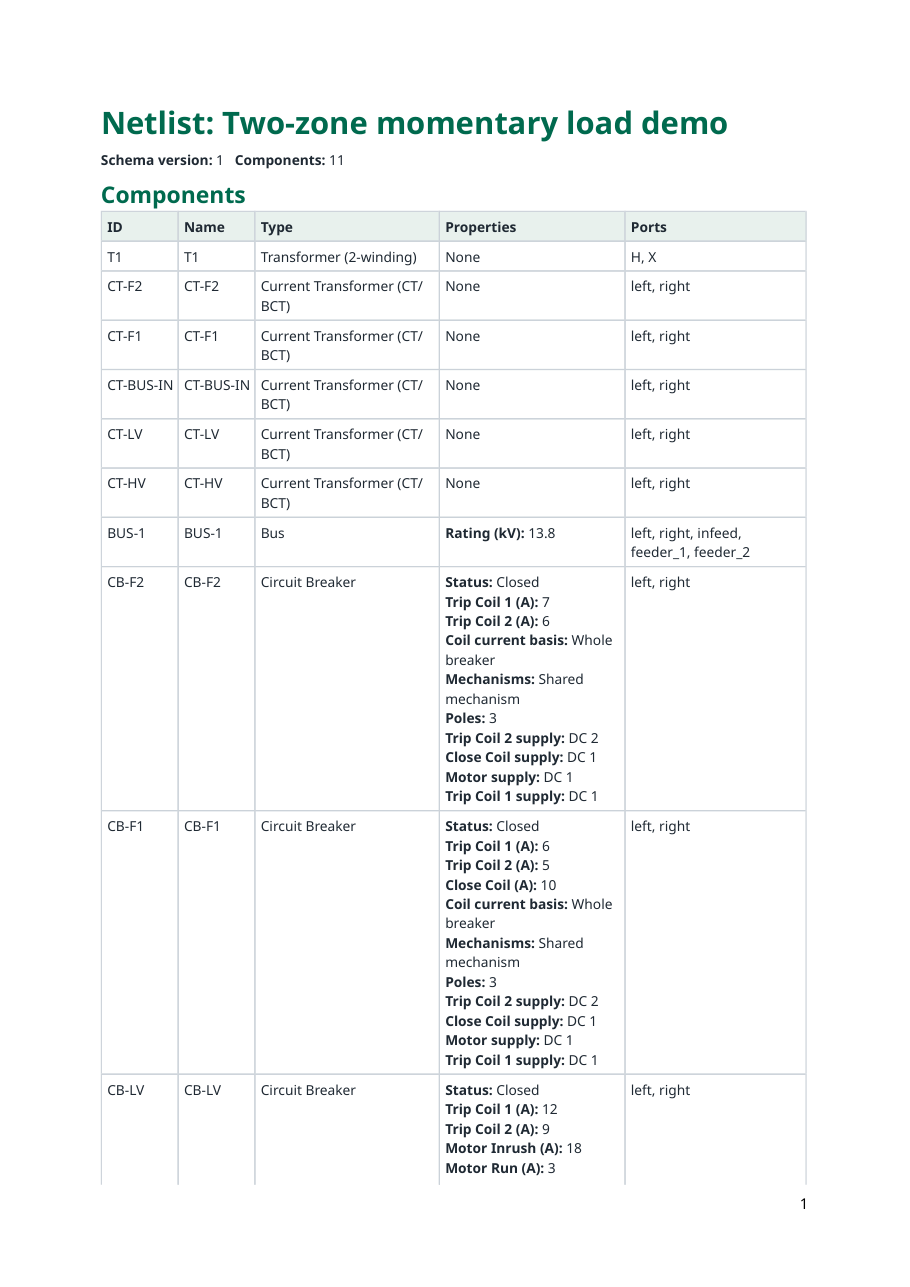
\includegraphics[width=0.46\textwidth]{images/netlist_pdf_p1.png}}
  \caption{First page of the netlist PDF for the two-zone demonstration}
  \label{fig:netlistpdf}
\end{figure}

% =====================================================================
\subsection{Provided One-Line Layouts}\label{sec:providedlayouts}

The project includes 12 layouts rebuilt from real one-line drawings, plus a small
demonstration (Table~\ref{tab:layouts}). The portable package contains the 12 real
layouts. Use them to learn the tool or as a starting point, bearing in mind that:


\begin{itemize}
  \item The breakers and motor-operated switches carry \emph{sample} currents, not
        manufacturer ratings.
  \item Each zone's breakers have both trip coils assigned in the Primary trip stage on
        DC 1. Closing, motor inrush and motor running are separate stages.
  \item Devices without a suggested zone have separate \emph{independent operation}
        scenarios. These do not represent additional protection zones.
  \item Except for the two-zone demonstration, the zones are not verified, so their
        results are provisional until reviewed.
\end{itemize}

\begin{table}[H]
  \centering
  \caption{Provided layouts}
  \label{tab:layouts}
  \begin{tabular}{l r r r r}
    \toprule
    \textbf{Layout} & \textbf{Components} & \textbf{Connections} & \textbf{Zones} & \textbf{Stages} \\
    \midrule
    1M-1L01 & 67 & 68 & 8 & 32 \\
    1P-1L01-Model & 51 & 51 & 5 & 14 \\
    1U-1L01-Layout1 & 80 & 80 & 11 & 44 \\
    1U-1L01-Model\_1 & 92 & 92 & 13 & 48 \\
    1U-1L01-Model\_5 & 52 & 51 & 6 & 24 \\
    1U-1L01\_1 & 34 & 33 & 7 & 16 \\
    A-089881-Layout1 & 9 & 8 & 2 & 8 \\
    A-89887-Layout1 & 44 & 46 & 6 & 24 \\
    AA-69925-Layout1 & 65 & 64 & 9 & 36 \\
    AS-1-Layout1 & 26 & 25 & 6 & 24 \\
    AS-11-Layout1 & 59 & 58 & 7 & 28 \\
    MVEC reference draft & 61 & 60 & 3 & 0 \\
    Two-zone demonstration & 14 & 13 & 2 & 5 \\
    \midrule
    \textbf{Total} & \textbf{654} & \textbf{649} & \textbf{85} & \textbf{303} \\
    \bottomrule
  \end{tabular}
\end{table}

The MVEC reference draft has its zones marked but no loads assigned. The two-zone
demonstration is fully verified and is the worked example in
Section~\ref{sec:workedexample}.
